\newpage
\subsection{UC3 - Modifica dei Metadati}
\label{sub:uc3}

\begin{figure}[h]
    \centering
    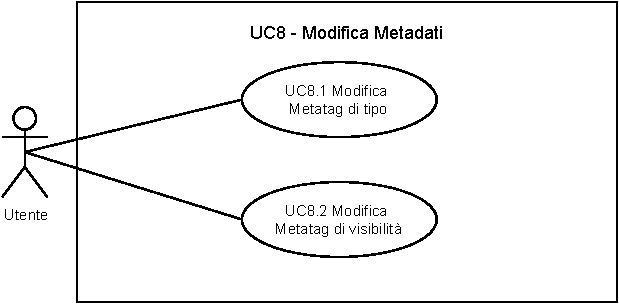
\includegraphics[width=0.7\textwidth]{componenti/casi-duso/diagrammi/UC3.pdf}
    \caption{Diagramma rappresentante UC3}
    \label{fig:UC3}
\end{figure}

%TODO: Al posto di cosi fare cosà:
        % Utente vuole modificare i metadati relativi ad una dimensione.
        % UTente sceglie dimensione. 
        % Utente modifca i metadati che preferisce.
\begin{itemize}
    \item \textbf{Descrizione}: L’utente vuole modificare un metadato attualmente assegnato ad una dimensione del dataset.
	
    \item \textbf{Attore primario}: Utente.
    
    \item \textbf{Precondizione}:   Nel programma è stato importato un dataset dotato di metadati per ogni sua dimensione.
    \item \textbf{Postcondizione}:  Vengono aggiornati i metadati della dimensione scelta dall'utente.

	\item \textbf{Scenario principale}:
        \begin{enumerate}
                \item L'utente sceglie una dimensione da modificare. (UC3.1)
                \item L'utente esegue le modifiche che preferisce tra quelle rese possibili. (UC3.2 e UC3.3)
                \item L'utente valida le modifiche apportate selezionando un pulsante di "Conferma".
        \end{enumerate}
    
    \item \textbf{Scenario alternativo}:
		\begin{enumerate}
			\item L'utente decide di annullare le modifiche selezionando il pulsante "Annulla". 
			\item Vengono ripristinati i metadati della dimensione precedenti alla modifica. (UC3.4)
        \end{enumerate}
\end{itemize}

\newpage

\subsubsection{UC3.1 - Scelta della dimensione da modificare}
\label{ssub:uc3.2}

\begin{itemize}
    \item \textbf{Descrizione}: L’utente seleziona una dimensione della quale modificare i metadati.	
    \item \textbf{Attore primario}: Utente.

    \item \textbf{Precondizione}:   L'utente ha aperto il menu di modifica dei metadati.
    \item \textbf{Postcondizione}:  Viene selezionata la dimensione del dataset da modificare.

	\item \textbf{Scenario principale}: L'utente sceglie una dimensione tra quelle del dataset corrente.
\end{itemize}

\subsubsection{UC3.2 - Modifica metadato di tipo}
\label{ssub:uc3.1}

\begin{itemize}
    \item \textbf{Descrizione}: L’utente vuole modificare il metadato di tipo attualmente assegnato 
                                alla dimensione del dataset da lui selezionata. Egli sceglie il nuovo valore tra le opzioni che gli vengono rese disponibili.
	
    \item \textbf{Attore primario}: Utente.
    
    \item \textbf{Precondizione}:   L'utente ha selezionato una dimensione del dataset  da modificare
                                    e la voce "modifica metadato di tipo" dal menu di modifica dei metadati.
    \item \textbf{Postcondizione}:  Viene aggiornato il metadato di tipo della dimensione selezionata.

	\item \textbf{Scenario principale}:
        L'utente imposta il nuovo tipo tra le opzioni possibili per la dimensione selezionata.
\end{itemize}


\subsubsection{UC3.3 - Modifica metadato di visibilità}
\label{ssub:uc3.2}

\begin{itemize}
    \item \textbf{Descrizione}: L’utente vuole modificare il metadato di visibilità attualmente 
                                assegnato alla dimensione del dataset da lui selezionata.
                                Egli sceglie se rendere la dimensione visibile o nascosta.
	
    \item \textbf{Attore primario}: Utente.
    
    \item \textbf{Precondizione}:   L'utente ha selezionato una dimensione del dataset da modificare
                                    e la voce "modifica metadato di visibilità" dal menu di modifica dei metadati.

    \item \textbf{Postcondizione}:  Viene aggiornato il metadato di visibilità della dimensione selezionata.

	\item \textbf{Scenario principale}: L'utente imposta la nuova impostazione di visibilità tra "visibile" e "nascosta".
\end{itemize}


\subsubsection{UC3.4 - Annulla modifiche dei metadati}
\label{ssub:uc3.4}

\begin{itemize}
    \item \textbf{Descrizione}: L’utente vuole annullare l'operazione di modifica dei metadati di una dimensione.
    \item \textbf{Attore primario}: Utente.
    
    \item \textbf{Precondizione}:   L'utente ha selezionato il modulo di modifica dei metadati e ha effettuato 
                                    modifiche ai metadati di una dimensione da lui scelta.
    \item \textbf{Postcondizione}:  Vengono ripristinati i metadati della dimensione scelta.

	\item \textbf{Scenario principale}: L'utente seleziona l'opzione di annullamento delle modifiche.
\end{itemize}


